\documentclass{beamer}
\usepackage{graphicx}
\usepackage{tikz}
\usetikzlibrary{arrows.meta}

\usetheme{CambridgeUS}
\title{Lenia - DAI project}
\author[Luca Lumetti]{Luca Lumetti}

\begin{document}

\frame{\titlepage}

\begin{frame}
\frametitle{What are Lenia?}
  Lenia is a particular kind of cellular automata, which is continuous in time,
  space and state. They differ from other cellular automata patterns in being
  geometric, fuzzy, resilient, adaptive, and rule-generic. They were
  first presented in the paper \emph{Lenia — Biology of Artificial Life} by
  \emph{Bert Wang-Chak Chan}.
\end{frame}

\begin{frame}
  \frametitle{Cellular automata}
  A cellular automata (CA) is a mathematical system where a grid of cells is
  evolved according to a set of local rules. By using simple rules, interesting
  patterns start to emerge and lead to complex phenomena. One of the most famous
  examples of CA is the Game of Life (GoL) developed by Conway in 1970.
\end{frame}

\begin{frame}
  \frametitle{Game of Life}
  In GoL we have a grid of cells, each of which can be either alive or dead. The
  rules of the game are simple and consider only a 3x3 neighborhood:
  \begin{itemize}
    \item Any live cell with fewer than two live neighbours dies, as if by
          underpopulation.
    \item Any live cell with two or three live neighbours lives on to the next
          generation.
    \item Any live cell with more than three live neighbours dies, as if by
          overpopulation.
    \item Any dead cell with exactly three live neighbours becomes a live cell,
          as if by reproduction.
  \end{itemize}
\end{frame}

\begin{frame}
  \frametitle{Game of Life}
  In other words, GoL can be seen as a CA with:
  \begin{itemize}
    \item a finite number of states (dead or alive)
    \item a finite neighborhood
    \item a finite time step, every cells immediately evolves to the next state
  \end{itemize}
  Can we generalize these finite properties to be continuous?
\end{frame}

\begin{frame}
  \frametitle{Definition of CA}
  Before we can generalize the rules of GoL, we need to define a CA
  mathematically. A CA is a tuple $\mathcal{A} = (\mathcal{L}, \mathcal{T},
  \mathcal{S}, \mathcal{N}, \phi)$ where $\mathcal{L}$ is the d-dimensional
  lattice of grid, $\mathcal{T}$ is the timeline, $\mathcal{S}$ is the state,
  $\mathcal{N} \subset \mathcal{L}$ is the neighborhood, $\phi :
  \mathcal{S}^{\mathcal{N}} \rightarrow \mathcal{S}$ is the update rule.\\
  With $\mathcal{A}^t : \mathcal{L} \rightarrow \mathcal{S}$ we define the
  collection of states over the whole grid at timestep $t$, while
  $\mathcal{A}^t(x)$ is the state of the cell $x \in \mathcal{L}$
\end{frame}

\begin{frame}
  \frametitle{Implementation of GoL}
  To implement GoL we follow a different path than usual, that will help us to
  generalize the CA in the future. Given a 2D grid of cells $\mathcal{L}$, we
  define a kernel $\mathcal{K}$ that will be convolved over each cell of
  $\mathcal{L}$.\\For GoL we define the following kernel
  \begin{equation}
    \mathcal{K} = \begin{array}{ccc}
      1 & 1 & 1\\
      1 & 0 & 1\\
      1 & 1 & 1
    \end{array}
  \end{equation}
  The first thing to compute is the so called \emph{potential distribution} $U^t$ for each cell $x \in \mathcal{L}$:
  \begin{equation}
    U^{t}(x) = \mathcal{K} * \mathcal{A}^t(x)
  \end{equation}
\end{frame}

\begin{frame}
  \frametitle{Implementation of GoL}
  The next step is to feed the potential distribution into a growth mapping
  function $G(x): \mathbb{R} \rightarrow [-1, +1]$, this gives as the
  \emph{growth distribution} $G^t$, which for GoL is defined as:
  \begin{equation}
    G^{t}(x) = \begin{cases}
      0 & \text{if } U^{t}(x) == 2\\
      +1 & \text{if } U^{t}(x) == 3\\
      -1 & \text{otherwise}
    \end{cases}
  \end{equation}
  Now we can finally update the grid of cells by adding the growth distribution
  and clipping everything to the two states ${0, 1}$:
  \begin{equation}\label{eq:gol-update}
    \mathcal{A}^{t+1}(x) = [\mathcal{A}^t(x) + G^{t}(x)]^1_0
  \end{equation}
\end{frame}

\begin{frame}
  \frametitle{Implementation of GoL}
  Basically the growth distribution $G^t$ tells us how each cells change in the next step, $0$ mean that it remains in the same state, $+1$ mean the cell is born, $-1$ mean that the cell died.
\end{frame}
% \begin{frame}
%   \frametitle{GoL}
%   Using the notation above, GoL can be defined as a CA with $\mathcal{L} = \mathbb{Z}^2$, $\mathcal{T} = \mathbb{Z}$, $\mathcal{S} = {0,1}$ and $\mathcal{N} = \begin{bmatrix} 1 & 1 & 1\\ 1 & 0 & 1\\ 1 & 1 & 1\\ \end{bmatrix}$.\\
%     The update rule thus can be written as:
%     % convolution of the neighborhood with the state
%     \begin{equation}
%       U^{t}(x) = \sum_{i=-1}^1 \sum_{j=-1}^1 A(x_{i,j})^t \cdot \mathcal{N}_{i,j}
%     \end{equation}
%     \begin{equation}
%       \phi(\mathcal{A}^t(x)) = \begin{cases}
%         1 & \text{if } \mathcal{A}^t(x) = 1 \text{ and } \mathcal{U}(x) = 2 \\
%         1 & \text{if } \mathcal{U}(x) = 3 \\
%         0 & \text{otherwise }
%       \end{cases}
%     \end{equation}
%     $U(x)$ is called the \emph{potential distribution} given by the convolution of the kernel with the grid.
% \end{frame}

\begin{frame}
  \frametitle{From GoL to Lenia}
  From now on, we will start from the Game of Life, and try to achieve
  continuous states, continuous time, and continuous space, one by one.
  The first thing that can be done is to update every cell just by a fraction
  $\Delta t$ of $G^t$, when $\Delta t \rightarrow 0$ we get continuous time.\\
  We change equation \ref{eq:gol-update} to:
  \begin{equation}\label{eq:gol-update-dt}
    \mathcal{A}^{t+1}(x) = [\mathcal{A}^t(x) + G^{t}(x)\Delta t]^1_0
  \end{equation}
\end{frame}

\begin{frame}
  \frametitle{From GoL to Lenia}
  This make sense only if the state can be continuous too instead of only
  ${0,1}$. Then let's change $\mathcal{S}$ to be continuous:\\
  \begin{equation}
    \mathcal{S} = [0,1]
  \end{equation}
  To make the space continuous, the convolution
  kernel is enlarged to radius R and defined to have a ring shape. As R approaches
  infinity, the space become continuous.
\end{frame}

\begin{frame}
  \frametitle{From GoL to Lenia}
  To make the ring shape and the growth function \emph{smooth} we can define them using the gaussian function:\\
  \begin{equation}
    \mathcal{K}(\mu, \sigma, x) = exp(-\frac{(x-\mu)^2}{2\sigma^2})
  \end{equation}
  \begin{equation}
    G^t(\mu, \sigma, x) = 2exp(-\frac{(x-\mu)^2}{2\sigma^2}) - 1
  \end{equation}
\end{frame}

\begin{frame}
  \frametitle{Lenia}
  We now have achieved continuos time, space and state. We can now start to look for creatures by setting random $G_\mu$, $G_\sigma$, $K_\mu$, $K_\sigma$ and also initializing the grid with random values between $0$ and $1$.
\end{frame}

\begin{frame}
  The first creature found by Bert Wang-Chak Chan was named \emph{Orbium}.
  By setting the parameters to $G_\mu = 0.15$, $G_\sigma = 0.015$, $K_\mu =
  0.5$, $K_\sigma = 0.15$, we can get a creature that is able to move and
  survive in the grid.
  \begin{figure}
    \begin{center}
      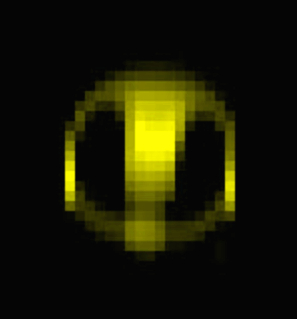
\includegraphics[width=0.2\textwidth]{./orbium.jpg}
    \end{center}
    \caption{Orbium}
  \end{figure}
\end{frame}

\begin{frame}
  \frametitle{Lenia}
  Different creature have been found just by initializing the parameters at random and playing with the grid:
  \begin{figure}
    \begin{center}
      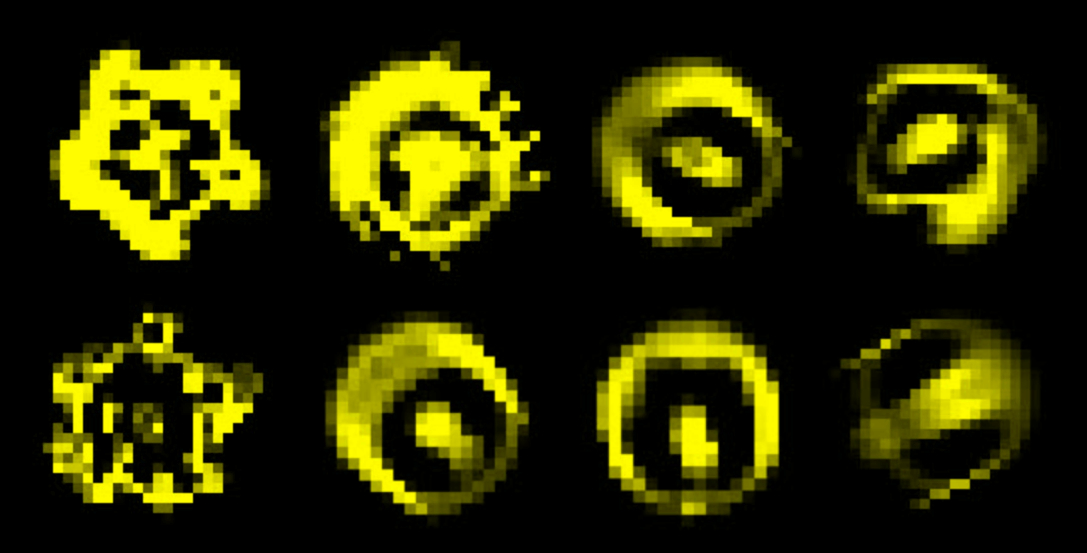
\includegraphics[width=0.6\textwidth]{./creatures.jpg}
    \end{center}
  \end{figure}
\end{frame}

\begin{frame}
  \frametitle{Extending Lenia}
  How can we push this further? We can actually use more that a single kernel,
  each one with a different growth function. Then we can weight the different
  growth distribution by a factor $h_i$. Then the formula became:
  \begin{equation}
    \mathcal{A}^{t+1}(x) = [\mathcal{A}^t(x) + \sum_{i=1}^N h_i G^t_i(U^t_i(x))\Delta t]^1_0
  \end{equation}
\end{frame}

\begin{frame}
  \frametitle{Extending Lenia}
  We can also add more grid and make them interact with each other by assigning
  to a kernel a source and a target. The source grid is the one that is used to
  compute $U^t$ and $G^t$ while the target grid is the one that will be updated.\\
  By using 3 grid, we can have RGB life-forms.
\end{frame}

\begin{frame}
  \frametitle{Extending Lenia}
  This obliviously gives us more parameters to tune and thus is harder to
  explore the whole parameters space and to find living creatures, but life-forms can
  exibith more complex behaviors such as self-replication, which was never been
  found in the "standard" Lenia.
  \begin{figure}
    \begin{center}
      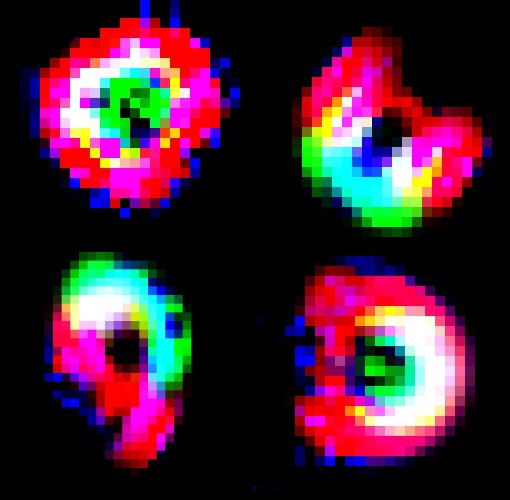
\includegraphics[width=0.4\textwidth]{./creatures_rgb.jpg}
    \end{center}
  \end{figure}
\end{frame}

\begin{frame}
  \frametitle{Extending Lenia}
  Until now, every cell relied on a global synchronous clock. We can now
  introduce a local clock to each cell and make the whole CA asynchronous.\\
  We can update a cell state with a probability of 50\%. Will the whole system
  still manage to self-organize and able to generate a living creature?
\end{frame}

\begin{frame}
  \frametitle{Extending Lenia}
  The answer is yes, the system is able to self-organize and some of the
  life-forms found in the synchronous Lenia can live in the asynchronous too. A
  drawback is that these life-forms are way more sensitive to noise.
  \begin{figure}
    \begin{center}
      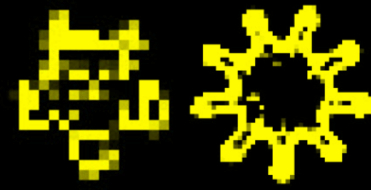
\includegraphics[width=0.4\textwidth]{./creatures_async.jpg}
    \end{center}
  \end{figure}

\end{frame}

\end{document}
